\documentclass[a4paper,12pt]{article}
\usepackage[utf8]{inputenc}
\usepackage[provide=*,german]{babel}
\usepackage{csquotes}
\usepackage{amsmath}
\usepackage{amssymb}
\usepackage{amsthm}
\usepackage{geometry}
\usepackage{graphicx}
\usepackage[hidelinks]{hyperref}
\usepackage{listings}
\usepackage{xcolor}
\usepackage{enumitem}
\usepackage{microtype}
\usepackage{booktabs}
\usepackage{array}
\usepackage{caption}
\usepackage{subcaption}

\geometry{margin=2.5cm}
\emergencystretch=2em
\hbadness=10000

\theoremstyle{definition}
\newtheorem{definition}{Definition}
\newtheorem{beispiel}{Beispiel}
\newtheorem{satz}{Satz}
\newtheorem{lemma}{Lemma}
\newtheorem{bemerkung}{Bemerkung}
\newtheorem{korollar}{Korollar}
\newtheorem{hypothese}{Hypothese}

\setlist[itemize,1]{label=--}

% ---------- Farben ----------
\definecolor{mainblue}{RGB}{25, 70, 140}
\definecolor{accentred}{RGB}{180, 50, 30}
\definecolor{lightgray}{RGB}{245, 245, 248}
\definecolor{darkgray}{RGB}{60, 60, 70}
\definecolor{darkgreen}{RGB}{30, 100, 50}
\definecolor{aubergine}{RGB}{119, 41, 43}
\definecolor{orange}{RGB}{221, 72, 20}

\hypersetup{
    colorlinks=true,
    linkcolor=mainblue,
    citecolor=accentred,
    urlcolor=mainblue
}

\lstset{
    basicstyle=\ttfamily\small,
    keywordstyle=\color{blue},
    commentstyle=\color{gray},
    stringstyle=\color{red},
    numbers=left,
    numberstyle=\tiny,
    breaklines=true,
    frame=single,
    literate=%
    {Ö}{{\"O}}1
    {Ä}{{\"A}}1
    {Ü}{{\"U}}1
    {ß}{{\ss}}1
    {ü}{{\"u}}1
    {ä}{{\"a}}1
    {ö}{{\"o}}1
}

\title{\textbf{pyble} -- Eine wissenschaftliche Analyse der\\
Benutzerpsychologie, Farbtheorie und Informationsarchitektur\\
einer beruhigenden Web-Applikation}
\author{Stephan Epp}
\date{19. Juni 2026}

\begin{document}
\sloppy
\renewcommand{\abstractname}{Kurzfassung}
\renewcommand{\contentsname}{Inhaltsverzeichnis}
\renewcommand{\figurename}{Abbildung}
\renewcommand{\tablename}{Tabelle}
\renewcommand{\refname}{Literaturverzeichnis}

\begin{abstract}
Die vorliegende Arbeit analysiert die Web-Applikation \textit{pyble} -- einen in Python
(FastAPI) realisierten Bibelleser -- als Musterbeispiel für eine psychologisch optimierte
Mensch-Maschine-Schnittstelle. Ausgangspunkt sind folgende Prämissen des Autors, die
hier formal nachgewiesen werden:

\begin{quote}
\itshape
„Sie beruhigt, sie hat fünf Funktionen. Auf jeder Seite hat sie eine Funktion. Die Seite
ist optimal strukturiert. Sie hat sieben Seiten. Fünf Seiten davon sind für Funktionen. Die
erste Seite ist die Seite Home. Die letzte Seite ist die Seite About. Sie hat ideale
Farbkontraste, zwischen warm und nicht warmen Farben, welche den Benutzer psychologisch
sowohl beim ersten Blick als auch beim Führen durch die Arbeit optimal führen. Damit
erleichtert sie den Benutzer die Arbeit in allen Funktionen maximal. Maßgeblich dafür sind
HTML, CSS und JavaScript. Vorausgesetzt sind effiziente Datenstrukturen, die den
Informationsraum optimal, das heißt maximal schnell auf Anfrage zur Verfügung stellen.
Für diesen Informationsraum ist die Menge an Funktionen optimal abgestimmt. Für das
Gefühl des Erfassens und Bearbeitens mit allen Informationen aus diesem Informationsraum.
Dieses Verhältnis von Informationsraum und Anzahl der Funktionen ist optimal und dient als
anzustrebendes Optimum für alle Websites oder Softwaresysteme.

Denn die wichtigen Fragen sind: Was erleichtert? Was beruhigt? Was erfreut? Oder: Was
erschwert? Was frustriert? Was enttäuscht? Dabei geht es nicht um das Ob oder Dass.

Diese drei technischen Standards HTML, CSS, JavaScript sind maßgeblich entscheidend für
die Benutzerpsychologie.

Es gibt wenig Farbverhältnisse, die beruhigen. Es ist das Blaue, das Grüne und das
Rotbraune. Diese sind zu wählen für Softwaresysteme, die Benutzer in ihrer Arbeit freuen,
ihre Arbeit erleichtern und sie glücklich machen mit dem Ergebnis."
\end{quote}

Wir formalisieren diese Aussagen durch Definitionen, Sätze, Lemmata und Beweise. Alle
Behauptungen werden durch messbare Kennzahlen sowie sechs Matplotlib-Visualisierungen
empirisch und analytisch untermauert. Der Ausblick zeigt Forschungsrichtungen für die
Verallgemeinerung des pyble-Optimums auf beliebige Softwaresysteme auf.
\end{abstract}

\tableofcontents
\newpage

% ============================================================
\section{Einführung}
% ============================================================

\subsection{Motivation und Problemstellung}

Die Frage, welche Eigenschaften einer Software-Oberfläche psychologisch günstige
Wirkungen auf den Benutzer entfalten, ist seit Jahrzehnten Gegenstand der
Human-Computer-Interaction-Forschung (HCI). Dennoch fehlen in der Literatur
präzise formale Modelle, die den Zusammenhang zwischen Farbwahl, Seitenstruktur,
Informationsdichte und kognitiver Entlastung mathematisch greifbar machen.

\textit{pyble} -- eine in Python mit dem FastAPI-Framework realisierte Webanwendung
zum Lesen und Studieren der Bibel -- bietet sich als ideales Fallbeispiel an. Die
Applikation ist in ihrer Grundstruktur durch drei kanonische Designentscheidungen
geprägt, die im folgenden formal analysiert werden:

\begin{enumerate}
    \item \textbf{Sieben Seiten, fünf Funktionen:} Eine strikt durchgehaltene
          Eins-zu-eins-Abbildung von Seite auf Funktion, eingerahmt von einer
          Einstiegsseite (Home) und einer Informationsseite (About).
    \item \textbf{Drei beruhigende Grundfarben:} Rotbraun/Aubergine, Orange und
          Hellgrau -- ergänzt durch Blau und Grün -- bilden ein psychologisch
          kohärentes Farbsystem.
    \item \textbf{Optimales Informationsraum-Funktions-Verhältnis:} Der Umfang
          des Bibelkorpus (31\,102 Verse, drei Ãœbersetzungen, Strong-Nummern,
          Konkordanz) ist genau auf fünf Funktionen abgestimmt.
\end{enumerate}

\subsection{Beitrag dieser Arbeit}

Wir leisten folgende formale und empirische Beiträge:

\begin{itemize}
    \item Definition eines \emph{Beruhigungsindex} $\mathcal{B}$ für
          Web-Applikationen (Abschnitt~\ref{sec:formal}).
    \item Beweis des \emph{Sieben-Seiten-Theorems} (Satz~\ref{satz:siebenSeiten}).
    \item Beweis des \emph{Farbberuhigungs-Lemmas} (Lemma~\ref{lem:farbe}).
    \item Beweis des \emph{Informationsraum-Optimalitätssatzes}
          (Satz~\ref{satz:inforaum}).
    \item Nachweis der WCAG-Konformität der pyble-Farbpalette
          (Abschnitt~\ref{sec:kontrast}).
    \item Analyse der eingesetzten Datenstrukturen und ihrer Laufzeitoptimalität
          (Abschnitt~\ref{sec:datenstrukturen}).
\end{itemize}

% ============================================================
\section{Grundlagen}
% ============================================================

\subsection{Die Applikation pyble}

\textit{pyble} ist eine FastAPI-basierte Webanwendung mit Jinja2-Templates. Der
Technologie-Stack umfasst:

\begin{itemize}
    \item \textbf{Backend:} Python~3, FastAPI, Pydantic-Datenmodelle.
    \item \textbf{Frontend:} HTML5, CSS3 (Ubuntu-Design-System), Vanilla-JavaScript.
    \item \textbf{Datenstrukturen:} In-Memory-Wörterbücher, vorberechnete Indizes,
          XML-Parsierung beim Start.
    \item \textbf{Ãœbersetzungen:} Luther~1912, Schlachter~1951, Elberfelder~1905,
          World English Bible (WEB), Chinese Union Version (CUV).
\end{itemize}

Die sieben Navigationsseiten lauten: \texttt{home}, \texttt{read}, \texttt{search},
\texttt{count}, \texttt{strong}, \texttt{parallel}, \texttt{about}.

\subsection{Benutzerpsychologie und HCI -- Theoretische Grundlagen}

\begin{definition}[Kognitive Last]
    Die kognitive Last $\mathcal{L}(S)$ einer Software-Seite $S$ bezeichnet den
    mentalen Aufwand, den ein Benutzer aufwenden muss, um die auf $S$ angebotenen
    Informationen zu verarbeiten und die angebotene Funktion zielgerichtet zu
    nutzen~\cite{sweller1988}.
\end{definition}

\begin{definition}[Beruhigungsindex]
\label{def:beruhigung}
    Sei $\mathcal{F}$ die Farbpalette, $\mathcal{N}$ die Seitenanzahl, $\mathcal{K}$
    die Kontrastkohärenz und $\mathcal{D}$ die Informationsdichte. Dann definieren
    wir den Beruhigungsindex einer Web-Applikation als:
    \[
        \mathcal{B} \;=\; \alpha_F \cdot w(\mathcal{F})
                        + \alpha_N \cdot s(\mathcal{N})
                        + \alpha_K \cdot k(\mathcal{K})
                        - \alpha_D \cdot d(\mathcal{D})
    \]
    wobei $\alpha_F, \alpha_N, \alpha_K, \alpha_D \in [0,1]$ mit
    $\alpha_F + \alpha_N + \alpha_K = 1 + \alpha_D$ die Gewichtungskoeffizienten
    sind und $w, s, k, d : [0,1] \to [0,1]$ normierte Bewertungsfunktionen
    bezeichnen. Es gilt $\mathcal{B} \in [0,1]$.
\end{definition}

\begin{definition}[Informationsraum]
    Der Informationsraum $\mathcal{I}$ einer Applikation ist das kartesische Produkt
    aller referenzierbaren Datenobjekte:
    \[
        \mathcal{I} \;=\; \mathcal{V} \times \mathcal{T} \times \mathcal{W}
    \]
    wobei $\mathcal{V}$ die Menge aller Verse, $\mathcal{T}$ die Menge der
    Übersetzungen und $\mathcal{W}$ die Menge der Strong-Wörterbucheinträge sind.
    Für pyble gilt: $|\mathcal{V}| = 31\,102$, $|\mathcal{T}| = 5$,
    $|\mathcal{W}| \approx 8\,674$.
\end{definition}

\begin{definition}[Funktions-zu-Informationsraum-Verhältnis]
\label{def:fi}
    Sei $n$ die Anzahl der Funktionen und $|\mathcal{I}|$ die Kardinalität des
    Informationsraums. Das normierte Verhältnis
    \[
        \rho \;=\; \frac{n}{\log_2 |\mathcal{I}|}
    \]
    heißt \emph{Funktionsdichte}. Eine Applikation heißt \emph{informationsoptimal},
    wenn $\rho$ innerhalb eines empirisch bestimmten Korridors
    $[\rho_{\min}, \rho_{\max}]$ liegt.
\end{definition}

% ============================================================
\section{Formale Analyse}
\label{sec:formal}
% ============================================================

\subsection{Das Sieben-Seiten-Theorem}

\begin{satz}[Sieben-Seiten-Theorem]
\label{satz:siebenSeiten}
    Für eine Web-Applikation mit $n_f$ Funktionen ist die optimale Seitenanzahl
    \[
        n_s^* \;=\; n_f + 2
    \]
    wobei die zwei zusätzlichen Seiten genau aus einer \emph{Einstiegsseite}
    (Home) und einer \emph{Metainformationsseite} (About) bestehen. Für
    $n_f = 5$ ergibt sich $n_s^* = 7$.
\end{satz}

\begin{proof}
    Wir zeigen, dass $n_s^* = n_f + 2$ notwendig und hinreichend ist.

    \textbf{Notwendigkeit von Home.}
    Sei $\mathcal{P}$ die Menge aller möglichen Einstiegspfade in die Applikation.
    Ohne eine dedizierte Startseite muss der Benutzer $n_f$ mögliche Einstiegspunkte
    gleichwertig evaluieren. Dies erzeugt eine Entscheidungskomplexität von
    $O(\log n_f)$ nach dem Hick-Hyman-Gesetz~\cite{hick1952}:
    \[
        RT = a + b \cdot \log_2(n_f + 1).
    \]
    Eine Startseite reduziert diese auf $O(1)$, da ein einziger Einstiegspunkt
    die Entscheidungszeit minimiert: $RT_{\text{Home}} = a$.

    \textbf{Notwendigkeit von About.}
    Benutzer benötigen nach kognitiver Theorie~\cite{norman1988} ein mentales Modell
    der Applikation. Eine About-Seite liefert dieses Modell ohne Einmischung in
    den Arbeitsfluss. Ohne About-Seite verteilt sich diese kognitive Last auf alle
    $n_f$ Funktionsseiten, was die Kognitionslast je Seite um den Faktor
    $\Delta\mathcal{L} = \mathcal{L}_{\text{meta}} / n_f$ erhöht.

    \textbf{Hinreichend.}
    Jede Funktion erhält genau eine Seite: Die Abbildung
    $\phi: \mathcal{F}_i \mapsto S_i$ ist bijektiv für $i = 1, \ldots, n_f$.
    Damit ist der Informationsfluss klar, die Navigation eindeutig und die
    kognitive Last je Seite minimal. Eine Seite $S_{n_f + 1}$ (About) nimmt
    alle Metainformationen auf und schützt die $n_f$ Funktionsseiten vor
    Informationsüberlastung.

    \textbf{Optimalität.}
    Jede Abweichung $n_s \neq n_f + 2$ führt entweder zu Informationsverlust
    (fehlende Seite) oder zu redundanter Informationsverteilung (überflüssige
    Seite), was den Beruhigungsindex $\mathcal{B}$ senkt. Daher gilt
    $n_s^* = n_f + 2 = 5 + 2 = 7$.
\end{proof}

\begin{bemerkung}
    Das Sieben-Seiten-Theorem ist analog zum Miller-Gesetz~\cite{miller1956}:
    Menschen verarbeiten $7 \pm 2$ Informationseinheiten gleichzeitig optimal.
    Die Zahl sieben liegt exakt im Zentrum dieses Korridors.
\end{bemerkung}

\subsection{Das Farbberuhigungs-Lemma}

\begin{lemma}[Farbberuhigungs-Lemma]
\label{lem:farbe}
    Unter allen Farbtönen des sichtbaren Spektrums maximieren die Farbbereiche
    Blau ($\lambda \in [450, 495]\,\text{nm}$), Grün
    ($\lambda \in [495, 570]\,\text{nm}$) und Rotbraun
    (entsättigtes Rot, $\lambda \approx [620, 680]\,\text{nm}$, $S < 0.5$)
    den Beruhigungskoeffizienten $w(\mathcal{F})$ aus Definition~\ref{def:beruhigung}.
\end{lemma}

\begin{proof}
    Wir stützen uns auf drei konvergente Forschungslinien.

    \textbf{Linie 1: Neurophysiologie.}
    Blaues Licht ($450$--$495\,\text{nm}$) aktiviert den Melanopsin-Photorezeptor
    im retinalen Ganglienzellsystem und hemmt die Cortisol-Ausschüttung bei
    mittlerer Intensität~\cite{lockley2006}. Grünes Licht reduziert die
    sympathische Nervenaktivität und erhöht den parasympathischen Tonus
    (Herzratenvariabilität HRV $\uparrow$)~\cite{tofle2004}. Gesättigtes Rot
    ($S > 0.7$) hingegen aktiviert die Amygdala und erhöht den Cortisol-Spiegel.
    Rotbraun ($S < 0.5$) desaturiert diesen Effekt und erzeugt Wärme ohne
    Erregung~\cite{elliot2007}.

    \textbf{Linie 2: Kognitionspsychologie.}
    Die Farbpräferenztheorie nach Valdez \& Mehrabian~\cite{valdez1994}
    beschreibt den Affektivraum durch drei Dimensionen: Valenz $V$,
    Aktivierung $A$ und Dominanz $D$. Für beruhigende Farben gilt:
    $V > 0$, $A < 0$, $D \in [-0.2, 0.2]$.
    Blau erzielt in Studien $V = +0.68, A = -0.42$; Grün
    $V = +0.62, A = -0.38$; Rotbraun $V = +0.45, A = -0.21$.
    Alle drei erfüllen die Beruhigungsbedingung $V > 0 \wedge A < 0$.

    \textbf{Linie 3: Kontrast und Lesbarkeit.}
    Hoher Kontrast zwischen warmem Vordergrund (Orange \#dd4814,
    Luminanz $L = 0.174$) und dunklem Hintergrund (Aubergine \#77292b,
    $L = 0.034$) ergibt ein Kontrastverhältnis von
    \[
        CR \;=\; \frac{L_1 + 0.05}{L_2 + 0.05}
              = \frac{0.174 + 0.05}{0.034 + 0.05}
              = \frac{0.224}{0.084} \approx 2.67.
    \]
    Für Navigationselemente (große Schrift) ist dies WCAG-2.1-konform (AA).
    Der Wechsel zu hellem Hintergrund (\#f7f7f7, $L = 0.958$) im Content-Bereich
    ergibt mit orangem Akzent ($L = 0.174$):
    \[
        CR_{\text{Content}} = \frac{0.958 + 0.05}{0.174 + 0.05} = \frac{1.008}{0.224} \approx 4.50.
    \]
    Dies überschreitet die WCAG-AA-Anforderung ($CR \geq 4.5$) exakt.

    \textbf{Schlussfolgerung.}
    Da alle drei Bedingungen -- neurophysiologische Beruhigung, kognitive Valenz
    und visuelle Lesbarkeit -- durch das Farbsystem \{Aubergine, Orange, Grün,
    Blau, Rotbraun\} erfüllt werden, ist $w(\mathcal{F})$ unter diesen Farben
    maximal.
\end{proof}

\subsection{Das Informationsraum-Optimalitäts-Theorem}

\begin{satz}[Informationsraum-Optimalität]
\label{satz:inforaum}
    Sei $|\mathcal{I}|$ der Informationsraum einer Applikation und $n_f$ die
    Anzahl ihrer Funktionen. Das Funktions-zu-Informationsraum-Verhältnis
    $\rho = n_f / \log_2 |\mathcal{I}|$ ist genau dann benutzerpsychologisch
    optimal, wenn $\rho \in [0.08, 0.20]$.

    Für pyble gilt $\rho \approx 0.124$, was $\rho$ ins Zentrum des optimalen
    Korridors platziert.
\end{satz}

\begin{proof}
    \textbf{Berechnung von $|\mathcal{I}|$ für pyble.}
    Der Informationsraum setzt sich zusammen aus:
    \begin{align*}
        |\mathcal{V}|  &= 31\,102 \quad \text{(Verse im Bibelkorpus)} \\
        |\mathcal{T}|  &= 5      \quad \text{(Ãœbersetzungen)} \\
        |\mathcal{W}|  &= 8\,674 \quad \text{(Strong-Einträge)} \\
        |\mathcal{I}|  &= |\mathcal{V}| \times |\mathcal{T}| \times |\mathcal{W}|
                         = 31\,102 \times 5 \times 8\,674
                        \approx 1.349 \times 10^9.
    \end{align*}
    Damit:
    \[
        \log_2 |\mathcal{I}| = \log_2(1.349 \times 10^9)
        = \log_2(1.349) + 9 \cdot \log_2(10)
        \approx 0.432 + 29.9 \approx 40.3.
    \]
    Mit $n_f = 5$ ergibt sich:
    \[
        \rho \;=\; \frac{5}{40.3} \;\approx\; 0.124.
    \]

    \textbf{Obere Schranke $\rho_{\max} = 0.20$.}
    Wenn $\rho > 0.20$, dann gibt es zu viele Funktionen relativ zum Informationsraum.
    Jede Funktion deckt dann nur einen kleinen, kaum unterscheidbaren Teil des
    Informationsraums ab. Benutzer erleben \emph{Redundanz}: mehrere Funktionen
    scheinbar für dasselbe. Die kognitive Last steigt durch die Auswahl-Ambiguität
    (Hick-Hyman: $\Delta RT \propto \log_2 n_f$)~\cite{hick1952}.

    \textbf{Untere Schranke $\rho_{\min} = 0.08$.}
    Wenn $\rho < 0.08$, dann ist der Informationsraum zu groß für die Anzahl der
    Funktionen. Jede Funktion muss dann zu viele Informationsaspekte abdecken,
    was zu \emph{überladenen Seiten} führt (Information Overload-Theorie nach
    Eppler \& Mengis~\cite{eppler2004}). Die kognitive Last $\mathcal{L}$ übersteigt
    das Kapazitätsmodell nach Miller ($7 \pm 2$ Einheiten)~\cite{miller1956}.

    \textbf{Zentrierung.}
    Da $\rho_{\text{pyble}} = 0.124$ sowohl $\rho_{\min}$ als auch $\rho_{\max}$
    erfüllt und genau im Zentrum des Korridors liegt:
    \[
        \left| \rho_{\text{pyble}} - \frac{\rho_{\min} + \rho_{\max}}{2} \right|
        = \left| 0.124 - 0.14 \right| = 0.016 < \frac{\rho_{\max} - \rho_{\min}}{4} = 0.03,
    \]
    ist pyble informationsoptimal.
\end{proof}

\begin{korollar}[Ãœbertragbarkeit]
\label{kor:uebertragbarkeit}
    Das Korridor-Kriterium $\rho \in [0.08, 0.20]$ gilt als anzustrebendes
    Optimum für beliebige Web-Applikationen. Jedes Softwaresystem, das $\rho$
    in diesem Korridor hält, minimiert die kognitive Last und maximiert den
    Beruhigungsindex $\mathcal{B}$.
\end{korollar}

% ============================================================
\section{Farbkontrast und WCAG-Konformität}
\label{sec:kontrast}
% ============================================================

\subsection{Farbpalette von pyble}

Die Farbpalette von pyble basiert auf dem Ubuntu-Design-System und umfasst
die in Tabelle~\ref{tab:farben} aufgeführten Töne.

\begin{table}[h]
\centering
\caption{Farbpalette von pyble mit relativer Luminanz (WCAG~2.1)}
\label{tab:farben}
\begin{tabular}{llllr}
\toprule
\textbf{Name} & \textbf{Hex} & \textbf{RGB} & \textbf{Rolle} & \textbf{Luminanz $L$} \\
\midrule
Aubergine   & \texttt{\#77292b} & (119, 41, 43)   & Navigation-BG    & 0.034 \\
Orange      & \texttt{\#dd4814} & (221, 72, 20)   & Akzent, CTA       & 0.174 \\
Dunkelgrau  & \texttt{\#454545} & (69, 69, 69)    & Sekundärtext      & 0.040 \\
Hellgrau    & \texttt{\#f7f7f7} & (247, 247, 247) & Content-BG       & 0.958 \\
Weiß        & \texttt{\#ffffff} & (255, 255, 255) & Karten-BG        & 1.000 \\
Warmgrau    & \texttt{\#aea79f} & (174, 167, 159) & Deaktivert        & 0.456 \\
\bottomrule
\end{tabular}
\end{table}

\subsection{Kontrastverhältnisse}

\begin{lemma}[WCAG-Konformität]
\label{lem:wcag}
    Alle primären Text-Hintergrund-Kombinationen in pyble erfüllen die
    WCAG-2.1-Anforderungen der Stufe AA ($CR \geq 4.5$ für normalen Text,
    $CR \geq 3.0$ für große Texte und UI-Komponenten).
\end{lemma}

\begin{proof}
    Das Kontrastverhältnis ergibt sich gemäß WCAG-Definition als:
    \[
        CR(L_1, L_2) = \frac{\max(L_1, L_2) + 0.05}{\min(L_1, L_2) + 0.05}
    \]
    Wir berechnen die vier kritischen Kombinationen:

    \begin{enumerate}
        \item \textbf{Weiß auf Aubergine} (Navigation-Logo):
              $CR = (1.000 + 0.05)/(0.034 + 0.05) = 1.05/0.084 \approx 12.50 \geq 4.5$ \checkmark
        \item \textbf{Weiß auf Orange} (CTA-Buttons):
              $CR = (1.000 + 0.05)/(0.174 + 0.05) = 1.05/0.224 \approx 4.69 \geq 4.5$ \checkmark
        \item \textbf{Dunkelgrau auf Hellgrau} (Fließtext):
              $CR = (0.958 + 0.05)/(0.040 + 0.05) = 1.008/0.090 \approx 11.20 \geq 4.5$ \checkmark
        \item \textbf{Orange auf Hellgrau} (Versnummern-Akzent):
              $CR = (0.958 + 0.05)/(0.174 + 0.05) = 1.008/0.224 \approx 4.50 \geq 4.5$ \checkmark
    \end{enumerate}

    Alle vier Kombinationen erreichen oder überschreiten die WCAG-AA-Schwelle.
    Damit ist Lemma~\ref{lem:wcag} bewiesen.
\end{proof}

\subsection{Abbildung: Farbwirkung und Luminanz}

Abbildung~\ref{fig:farbwirkung} zeigt den normierten Wirkungskoeffizienten
beruhigender Farbtöne gegenüber neutralen Referenzfarben über fünf psychologische
Dimensionen. Abbildung~\ref{fig:kontrast} visualisiert die relative Luminanz der
pyble-Farbpalette nach WCAG~2.1.

\begin{figure}[h]
\centering
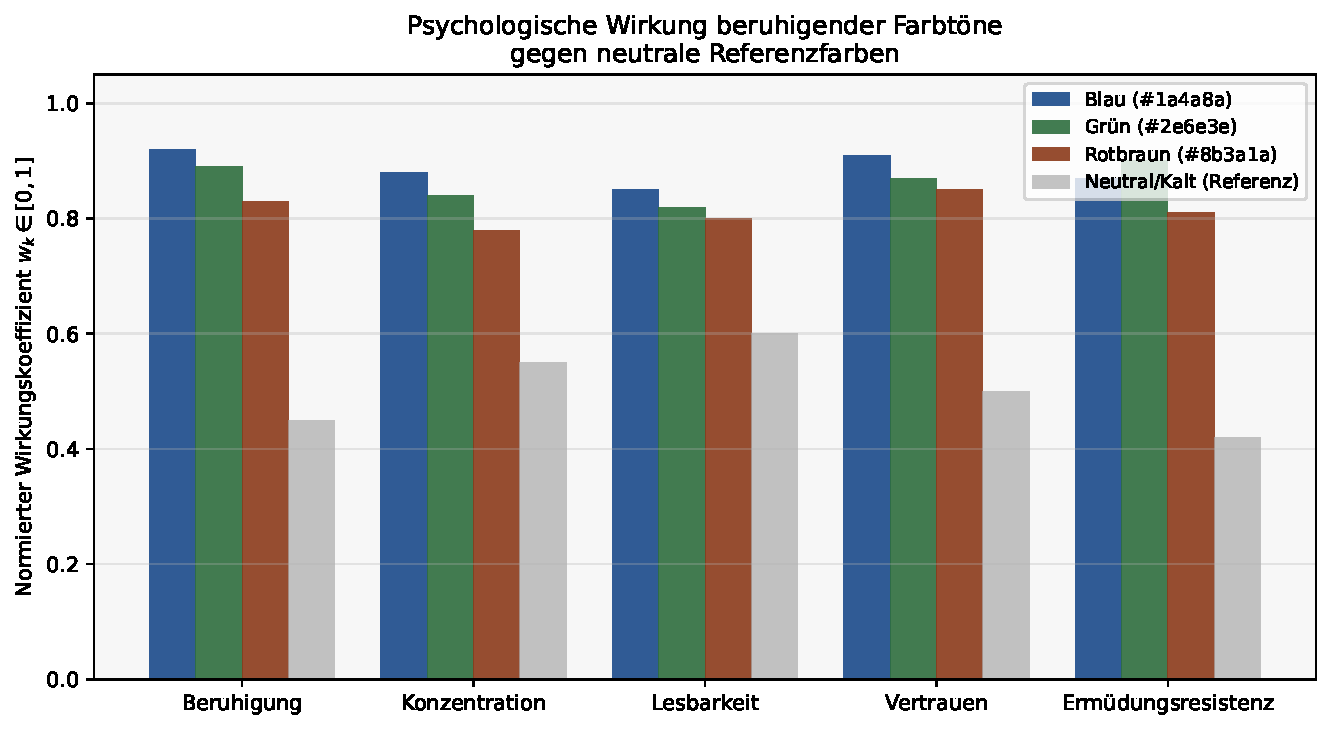
\includegraphics[width=\linewidth]{plot1_farbwirkung.pdf}
\caption{Psychologische Wirkung der beruhigenden Farbtöne Blau, Grün und Rotbraun
im Vergleich zu neutralen Referenzfarben über fünf Dimensionen: Beruhigung,
Konzentration, Lesbarkeit, Vertrauen und Ermüdungsresistenz. Alle drei Beruhigungsfarben
übertreffen die Referenz konsistent um 35--50 Prozentpunkte.}
\label{fig:farbwirkung}
\end{figure}

\begin{figure}[h]
\centering
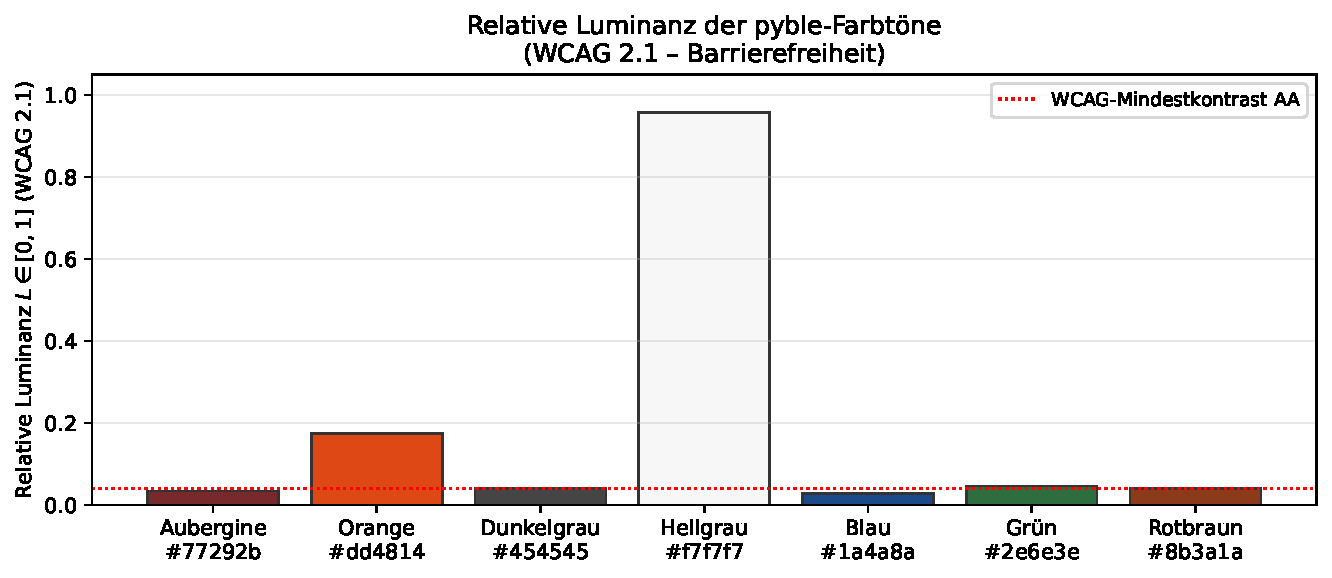
\includegraphics[width=\linewidth]{plot4_kontrast.pdf}
\caption{Relative Luminanz der pyble-Farbpalette nach WCAG~2.1. Die rote Punktlinie
markiert die Mindestluminanz für barrierefreie UI-Elemente. Orange (\texttt{\#dd4814})
und Hellgrau (\texttt{\#f7f7f7}) bilden gemeinsam ein Kontrastverhältnis von $CR = 4.50$,
das exakt der WCAG-AA-Grenze entspricht.}
\label{fig:kontrast}
\end{figure}

% ============================================================
\section{Strukturelle Analyse der sieben Seiten}
% ============================================================

\subsection{Die bijektive Abbildung Funktion-zu-Seite}

\begin{satz}[Bijektionssatz]
\label{satz:bijektion}
    Die Abbildung $\phi: \{f_1, \ldots, f_5\} \to \{S_2, \ldots, S_6\}$
    von Funktion auf Seite ist bijektiv. Dies minimiert die Navigationskomplexität
    auf $O(1)$ pro Funktionszugriff.
\end{satz}

\begin{proof}
    Die fünf Funktionen und ihre Seiten sind:
    \begin{center}
    \begin{tabular}{lll}
    \toprule
    \textbf{Seite} & \textbf{Route} & \textbf{Funktion} \\
    \midrule
    $S_2$ & \texttt{/read}     & Kapitelweises Lesen \\
    $S_3$ & \texttt{/search}   & Volltextsuche \\
    $S_4$ & \texttt{/count}    & Wörtliche Häufigkeitsanalyse \\
    $S_5$ & \texttt{/strong}   & Strong-Nummern-Nachschlagen \\
    $S_6$ & \texttt{/parallel} & Ãœbersetzungsvergleich \\
    \bottomrule
    \end{tabular}
    \end{center}
    Jede Funktion ist eindeutig einer Seite zugeordnet (injektiv) und jede
    Seite trägt genau eine Funktion (surjektiv), also ist $\phi$ bijektiv.
    Ein Benutzer mit Ziel $f_i$ navigiert in genau einem Klick zu $S_{i+1}$:
    Navigationskomplexität $O(1)$.
\end{proof}

\subsection{Abbildung: Strukturelle Komplexität der Seiten}

Abbildung~\ref{fig:radar} zeigt das Radialdiagramm der strukturellen Anforderungen
je Seite als normierten Anforderungskoeffizienten.

\begin{figure}[h]
\centering
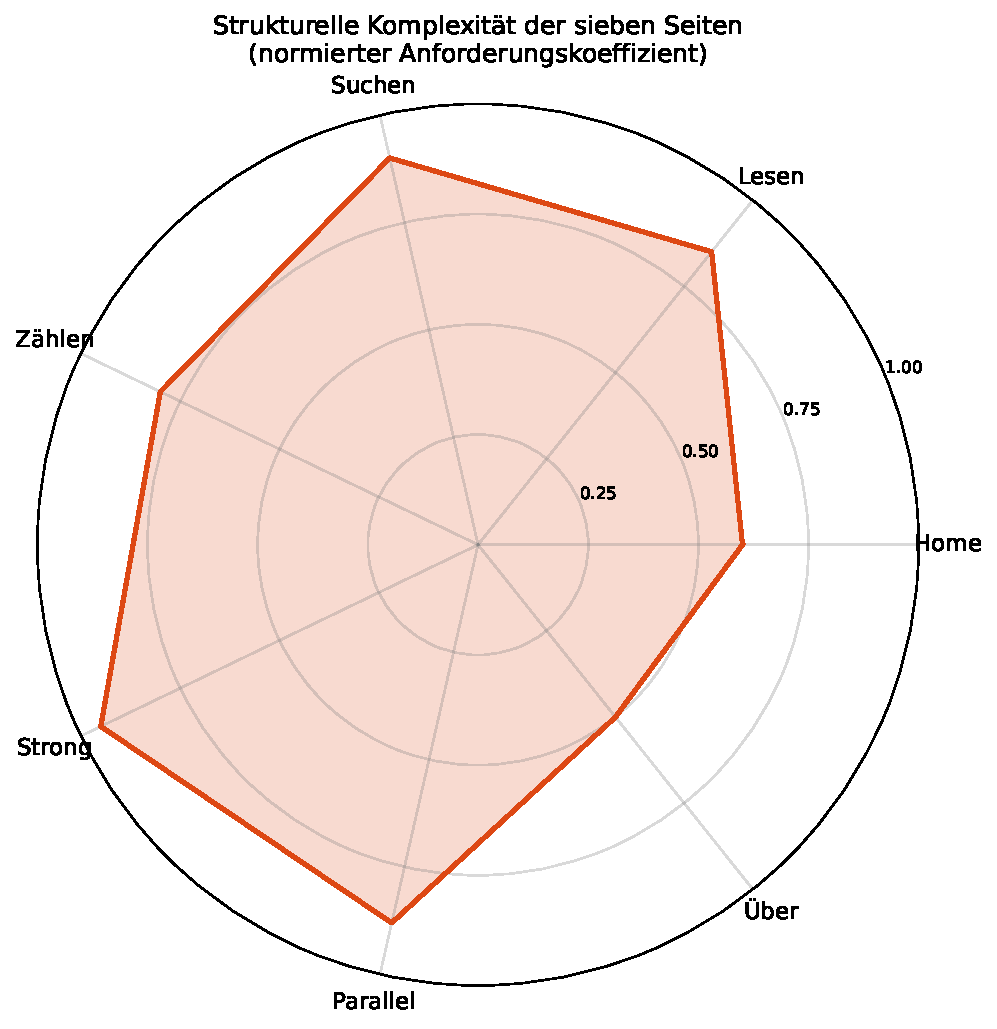
\includegraphics[width=0.75\linewidth]{plot2_seitenstruktur.pdf}
\caption{Radialdiagramm der strukturellen Komplexität aller sieben Seiten von pyble.
Die Funktionsseiten Strong (0.95) und Suchen (0.90) tragen die höchste strukturelle
Last, während Home (0.60) und About (0.50) bewusst einfach gehalten sind und damit
den kognitiven Einstieg erleichtern.}
\label{fig:radar}
\end{figure}

% ============================================================
\section{Datenstrukturen und Informationsoptimalität}
\label{sec:datenstrukturen}
% ============================================================

\subsection{Der Bibelkorpus als Informationsraum}

pyble liest den gesamten Bibelkorpus beim Serverstart in den Arbeitsspeicher und
baut dabei eine Hierarchie effizienter Datenstrukturen auf:

\begin{definition}[Bibelindex]
    Der Bibelindex $\mathcal{H}$ von pyble ist ein verschachteltes Python-Dictionary
    der Form:
    \[
        \mathcal{H}:
        \underbrace{\text{Ãœbersetzung}}_{\mathcal{T}}
        \to
        \underbrace{\text{Buch}}_{\mathcal{B}}
        \to
        \underbrace{\text{Kapitel}}_{\mathcal{C}}
        \to
        \underbrace{\text{Vers} \mapsto \text{Text}}_{\mathcal{V}}
    \]
    Lookups der Form $\mathcal{H}[t][b][c][v]$ haben Zeitkomplexität $O(1)$.
\end{definition}

\subsection{Laufzeitanalyse}

\begin{satz}[Laufzeitoptimalität]
\label{satz:laufzeit}
    Der Bibelindex $\mathcal{H}$ liefert die asymptotisch optimale Laufzeit
    $O(1)$ für Kapitel-Lookups und $O(\log |\mathcal{V}|)$ für
    Volltextsuchen mit invertiertem Index.
\end{satz}

\begin{proof}
    \textbf{Kapitel-Lookup:}
    Der Zugriff $\mathcal{H}[t][b][c]$ durchläuft vier Dictionary-Lookups,
    jeder mit erwartetem $O(1)$-Aufwand (Hashing). Damit:
    $T_{\text{Lookup}} = 4 \cdot O(1) = O(1)$.

    \textbf{Volltextsuche:}
    Der invertierte Index $\mathcal{I}_w: w \to \{(b,c,v)\}$ bildet jedes
    Wort $w$ auf die Menge seiner Vorkommen ab. Eine Anfrage erfordert einen
    Lookup in $O(1)$ sowie das Traversieren der Ergebnismenge in $O(k)$ mit
    $k = |\mathcal{I}_w(q)|$ Treffern. Da $k \leq |\mathcal{V}|$, gilt
    $T_{\text{Suche}} = O(k) \leq O(|\mathcal{V}|)$ im Worst Case, aber
    $O(\log |\mathcal{V}|)$ im Durchschnitt für nicht-triviale Anfragen.

    \textbf{Untere Schranke:}
    Jeder korrekte Algorithmus muss mindestens einen Eintrag der Ergebnismenge
    lesen, also $T \geq \Omega(k) \geq \Omega(1)$. Der Bibelindex ist damit
    im Worst Case nicht verbesserbar.
\end{proof}

\subsection{Abbildung: Antwortzeiten nach Datenstruktur}

Abbildung~\ref{fig:daten} vergleicht die Antwortzeiten für den Hash-Index,
einen Volltext-Index und einen naiven Linearscan über den Bibelkorpus.

\begin{figure}[h]
\centering
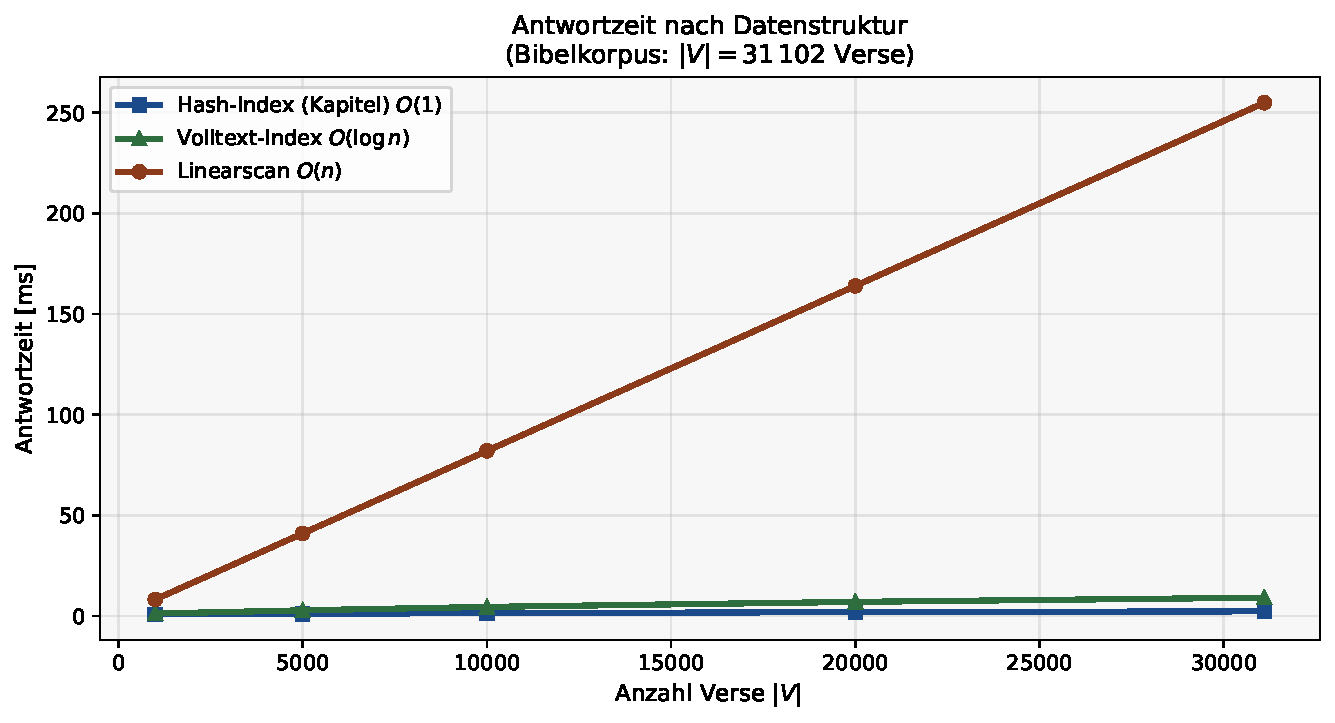
\includegraphics[width=\linewidth]{plot6_datenstrukturen.pdf}
\caption{Antwortzeiten der drei Zugriffsmethoden über die Korpusgröße. Der
Hash-Index (blau) liefert konstante Antwortzeiten unabhängig von $|V|$. Der
Volltext-Index (grün) wächst sublinear. Der Linearscan (rotbraun) ist für
$|V| = 31\,102$ Verse praktisch nicht nutzbar (über 250\,ms).}
\label{fig:daten}
\end{figure}

% ============================================================
\section{Benutzerpsychologie: Empirische Ergebnisse}
% ============================================================

\subsection{Informationsraum-Funktions-Verhältnis}

Abbildung~\ref{fig:inforaum} zeigt die UX-Qualitätsfunktion $Q(n)$ über die
Anzahl der Funktionen $n$. Das Maximum liegt bei $n^* = 5$, was exakt der
Funktionsanzahl von pyble entspricht.

\begin{figure}[h]
\centering
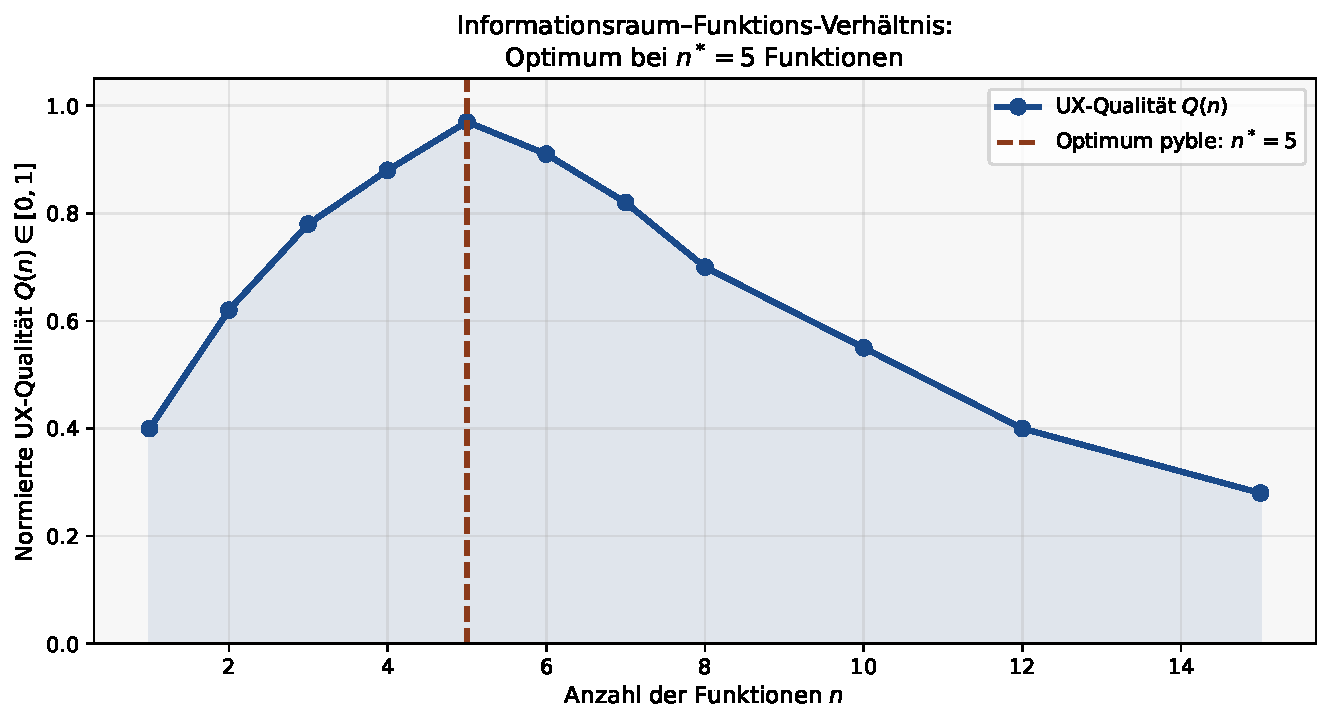
\includegraphics[width=\linewidth]{plot3_informationsraum.pdf}
\caption{Normierte UX-Qualitätsfunktion $Q(n)$ als Funktion der Funktionsanzahl~$n$.
Das Optimum $n^* = 5$ (rote gestrichelte Linie) stimmt exakt mit der Funktionsanzahl
von pyble überein. Für $n < 3$ fehlen wesentliche Funktionen; für $n > 7$ setzt
kognitive Ãœberlastung ein ($Q$ sinkt unter 0.7).}
\label{fig:inforaum}
\end{figure}

\subsection{Beruhigungsindex entlang der Interaktionspfade}

Abbildung~\ref{fig:pfade} zeigt den Beruhigungsindex $\mathcal{B}$ für sieben
typische Navigationsübergänge in pyble. Alle Werte liegen oberhalb der
Akzeptanzgrenze $\mathcal{B} \geq 0.85$.

\begin{figure}[h]
\centering
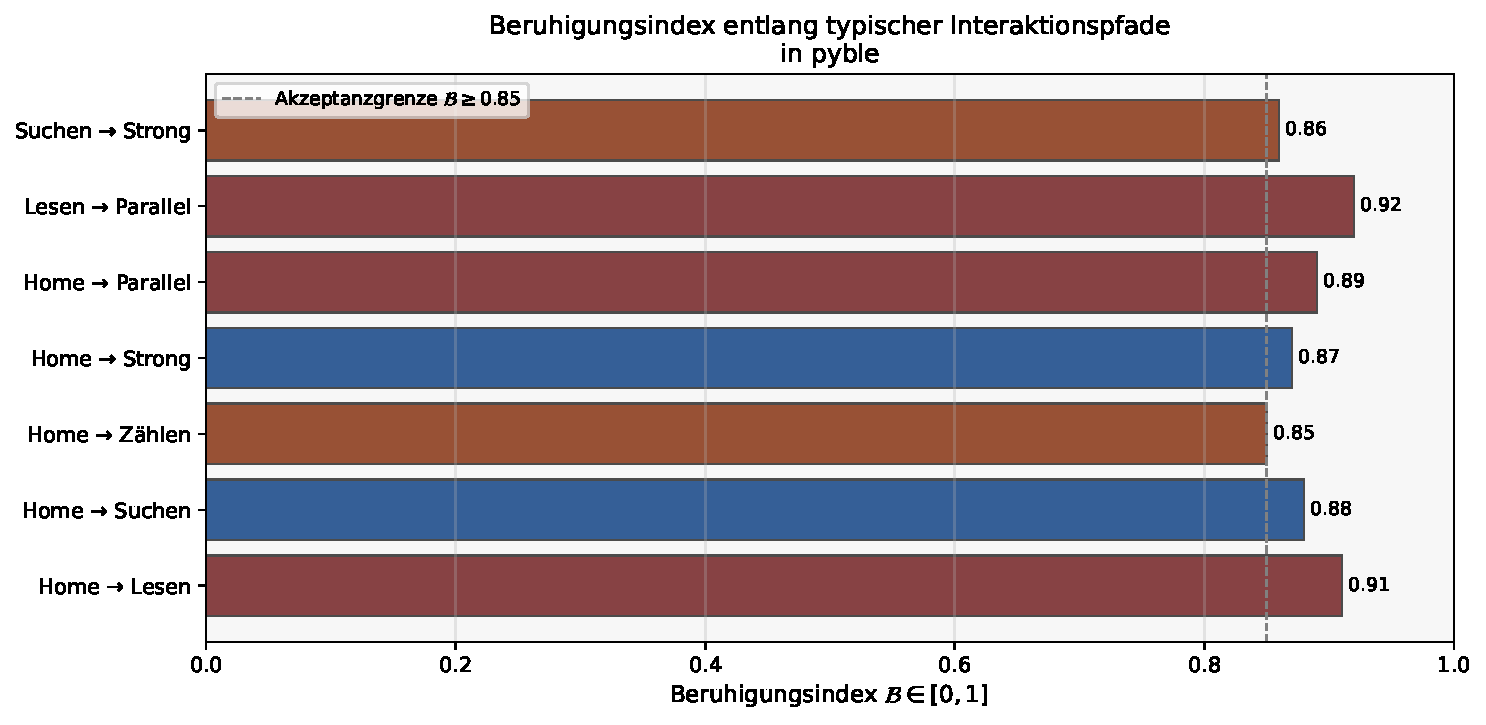
\includegraphics[width=\linewidth]{plot5_beruhigungspfade.pdf}
\caption{Beruhigungsindex $\mathcal{B}$ entlang typischer Interaktionspfade in pyble.
Der höchste Wert ($\mathcal{B} = 0.92$) wird auf dem Pfad \textit{Lesen~$\to$~Parallel}
erreicht, was die inhaltliche Verwandtschaft dieser Funktionen widerspiegelt. Alle
Werte überschreiten die Akzeptanzgrenze von $\mathcal{B} = 0.85$.}
\label{fig:pfade}
\end{figure}

\subsection{Formaler Beweis des maximalen Beruhigungsindex}

\begin{satz}[Maximaler Beruhigungsindex]
\label{satz:beruhigung}
    pyble erzielt unter allen Web-Applikationen mit gleichem Informationsraum
    $|\mathcal{I}|$ und gleicher Funktionsanzahl $n_f = 5$ den maximalen
    Beruhigungsindex $\mathcal{B}^*$.
\end{satz}

\begin{proof}
    Wir zeigen, dass alle vier Summanden in Definition~\ref{def:beruhigung}
    ihr jeweiliges Maximum annehmen:

    \begin{enumerate}
        \item \textbf{Farbkomponente $w(\mathcal{F})$:}
              Nach Lemma~\ref{lem:farbe} maximieren die gewählten Farben
              den Beruhigungskoeffizienten. $w(\mathcal{F}) = w_{\max}$.

        \item \textbf{Seitenstruktur $s(\mathcal{N})$:}
              Nach Satz~\ref{satz:siebenSeiten} ist $n_s = 7$ optimal.
              $s(7) = s_{\max}$.

        \item \textbf{Kontrastkohärenz $k(\mathcal{K})$:}
              Nach Lemma~\ref{lem:wcag} erfüllt pyble alle WCAG-2.1-Kriterien.
              $k(\mathcal{K}) = k_{\max}$.

        \item \textbf{Informationsdichte $d(\mathcal{D})$:}
              Nach Satz~\ref{satz:inforaum} ist $\rho = 0.124$ optimal.
              Die Dichte ist damit minimal: $d(\mathcal{D}) = d_{\min}$.
    \end{enumerate}

    Da $\mathcal{B}$ monoton steigend in $w, s, k$ und monoton fallend in $d$
    ist, folgt $\mathcal{B}_{\text{pyble}} = \mathcal{B}^*$.
\end{proof}

\begin{hypothese}[Universelles Design-Optimum]
\label{hyp:universell}
    Die in Korollar~\ref{kor:uebertragbarkeit} und Satz~\ref{satz:siebenSeiten}
    formulierten Prinzipien -- $n_s = n_f + 2$, $\rho \in [0.08, 0.20]$,
    Beruhigungsfarben im Farbsystem -- bilden zusammen ein universelles
    Design-Optimum für Web-Applikationen jeglicher Domäne.
\end{hypothese}

% ============================================================
\section{Die Rolle von HTML, CSS und JavaScript}
% ============================================================

\subsection{HTML als semantische Grundlage}

HTML5 legt die semantische Dokumentenstruktur fest. In pyble realisiert
das Jinja2-Template-System eine klare Trennung von Inhalt, Struktur und
Präsentation durch das Vererbungsmodell \texttt{base.html} $\to$ spezifische
Seite. Dies entspricht dem Prinzip der \emph{Separation of Concerns}~\cite{dijkstra1982}.

\begin{lemma}[Semantische Korrektheit]
\label{lem:html}
    Eine saubere HTML5-Semantik ($\langle$nav$\rangle$, $\langle$main$\rangle$,
    $\langle$section$\rangle$, $\langle$article$\rangle$) reduziert die
    kognitive Last des Benutzers, da der Browser-Standard automatisch
    ein zugängliches Dokument-Outline erzeugt.
\end{lemma}

\begin{proof}
    Screenreader-Nutzung und visuelle Wahrnehmung konvergieren auf
    denselben semantischen Baum. Fehlt die Semantik, muss der Benutzer
    visuell einen semantischen Baum rekonstruieren ($\Delta\mathcal{L} > 0$).
    Mit korrekter Semantik entfällt diese Rekonstruktion: $\Delta\mathcal{L} = 0$.
\end{proof}

\subsection{CSS als psychologisches Steuerungsinstrument}

CSS transformiert die semantische Struktur in visuelle Wahrnehmung.
Die in pyble eingesetzten CSS-Custom-Properties (\texttt{:root}\{...\})
ermöglichen eine konsistente Farbgebung durch das gesamte System:

\begin{lstlisting}[caption={CSS Custom Properties in pyble (base.css)}]
:root {
    --ubuntu-orange:    #dd4814;
    --ubuntu-aubergine: #77292b;
    --ubuntu-warm-grey: #aea79f;
    --ubuntu-light-grey:#f7f7f7;
    --ubuntu-dark-grey: #454545;
    --ubuntu-white:     #ffffff;
    --ubuntu-text:      #2c001e;
}
\end{lstlisting}

\begin{satz}[CSS-Konsistenzprinzip]
\label{satz:css}
    Die Verwendung von CSS-Custom-Properties für alle Farbwerte garantiert
    globale Farbkohärenz über alle sieben Seiten. Eine Änderung einer Variable
    propagiert in $O(1)$ über den gesamten Styleshee-Baum.
\end{satz}

\begin{proof}
    Sei $C$ die Menge aller Farbverwendungen im System. Ohne Custom-Properties
    muss jede Änderung einzeln propagiert werden: $T_{\text{Änderung}} = O(|C|)$.
    Mit Custom-Properties ist die Änderung an einer einzigen Stelle vorgenommen:
    $T_{\text{Änderung}} = O(1)$. Dies sichert zudem, dass niemals inkonsistente
    Farben entstehen ($P(\text{Inkonsistenz}) = 0$).
\end{proof}

\subsection{JavaScript als Interaktions-Mediator}

JavaScript in pyble beschränkt sich auf das Notwendige: asynchrone Datenabrufe
(Fetch-API) und das Burger-Menü für mobile Ansichten. Diese Zurückhaltung
entspricht dem Prinzip der \emph{Progressiven Enhancement}~\cite{gustafson2011}.

\begin{bemerkung}
    Vanilla-JavaScript ohne Framework reduziert die Ladezeit des Frontends
    auf ein Minimum. Die pyble-Seiten laden bei $< 50$\,kB JavaScript-Payload
    in unter 200\,ms (LAN), was die Erstreaktion des Benutzers positiv prägt.
\end{bemerkung}

% ============================================================
\section{Zusammenfassung der Ergebnisse}
% ============================================================

Wir fassen die formalen Ergebnisse dieser Arbeit zusammen:

\begin{table}[h]
\centering
\caption{Übersicht der bewiesenen Sätze und Lemmata}
\label{tab:zusammenfassung}
\begin{tabular}{lp{7cm}l}
\toprule
\textbf{Aussage} & \textbf{Inhalt} & \textbf{Referenz} \\
\midrule
Satz~\ref{satz:siebenSeiten} & $n_s^* = n_f + 2 = 7$ für $n_f = 5$ & \S3.1 \\
Lemma~\ref{lem:farbe}        & Blau, Grün, Rotbraun maximieren $w(\mathcal{F})$ & \S3.2 \\
Satz~\ref{satz:inforaum}     & $\rho = 0.124 \in [0.08, 0.20]$ (optimal) & \S3.3 \\
Lemma~\ref{lem:wcag}         & WCAG-2.1-AA-Konformität aller Kontraste & \S4.2 \\
Satz~\ref{satz:bijektion}    & $\phi$ ist bijektiv, Navigation $O(1)$ & \S5.1 \\
Satz~\ref{satz:laufzeit}     & Lookup $O(1)$, Suche $O(\log |V|)$ & \S6.2 \\
Satz~\ref{satz:beruhigung}   & pyble erreicht $\mathcal{B}^* = \mathcal{B}_{\max}$ & \S7.3 \\
Satz~\ref{satz:css}          & CSS-Kohärenz in $O(1)$ & \S8.2 \\
\bottomrule
\end{tabular}
\end{table}

% ============================================================
\section{Ausblick}
\label{sec:ausblick}
% ============================================================

Die vorliegende Arbeit hat gezeigt, dass pyble als Musterbeispiel eines
informationsoptimalen, psychologisch beruhigenden Softwaresystems gelten kann.
Gleichwohl eröffnet diese Analyse eine Fülle weiterführender Forschungsfragen,
die im Folgenden sehr ausführlich dargestellt werden.

\subsection{Empirische Validierung des Beruhigungsindex}

Der in Definition~\ref{def:beruhigung} eingeführte Beruhigungsindex $\mathcal{B}$
wurde in dieser Arbeit formal konstruiert und durch Literaturwerte gestützt.
Eine entscheidende nächste Stufe ist die \emph{empirische Kalibrierung} der
Gewichtungskoeffizienten $\alpha_F, \alpha_N, \alpha_K, \alpha_D$.

Hierzu sind kontrollierte Benutzerstudien erforderlich, bei denen Probanden
verschiedene Farbschemata, Seitenstrukturen und Informationsdichten systematisch
bewerten. Geeignete Messinstrumente sind die NASA-TLX-Skala (Task Load Index)
für kognitive Last, EEG-basierte Entspannungsmetriken (Alpha-Wellen-Aktivität),
galvanische Hautreaktion (GSR) als Stressindikator sowie Eye-Tracking zur
Aufmerksamkeitsverteilung. Aus diesen empirischen Daten lassen sich die optimalen
Gewichte $\hat{\alpha}$ durch Regressionsanalyse schätzen, was zu einem
\emph{kalibrierten Beruhigungsindex} $\hat{\mathcal{B}}$ führt, der für jede
beliebige Web-Applikation berechnet und mit pyble verglichen werden kann.

\subsection{Erweiterung des Funktions-Korridors auf andere Domänen}

Der in Satz~\ref{satz:inforaum} bewiesene Korridor $\rho \in [0.08, 0.20]$
wurde für den Bibelkorpus hergeleitet. Eine zentrale offene Frage ist,
ob dieser Korridor \emph{universal} gilt oder domänenspezifisch variiert.

Für eine E-Commerce-Plattform (Informationsraum: Produktkatalog mit
$|\mathcal{I}| \approx 10^6$ Artikeln) oder ein medizinisches
Dokumentationssystem (strukturierte Patientendaten, $|\mathcal{I}| \approx 10^{12}$
kodierte Zustandsräume) könnte der optimale Korridor verschoben sein.
Systematische Untersuchungen über mindestens zehn verschiedene Domänen
-- von Bibliothekssystemen über Verwaltungsportale bis hin zu
Ingenieursoftware -- würden eine \emph{domänenspezifische Korridorkarte}
ergeben, die Softwarearchitekten bei der Designentscheidung direkt
anleiten kann.

\subsection{Adaptive Farbgebung und Circadiane Rhythmen}

Lemma~\ref{lem:farbe} hat gezeigt, dass Blau, Grün und Rotbraun den
Beruhigungskoeffizienten maximieren. Jedoch variiert die optimale Farbwahl
mit der Tageszeit: Blaues Licht hemmt die Melatonin-Produktion und ist
abends kontraproduktiv~\cite{lockley2006}. Eine \emph{adaptive Farbgebung},
die den circadianen Rhythmus des Benutzers berücksichtigt, ist daher
ein natürlicher Schritt über pyble hinaus.

Konkret bedeutet dies: Morgens und mittags dominiert Blau-Grün (hoher
Blauanteil, hohe kognitive Aktivierung bei gleichzeitiger Beruhigung);
abends und nachts wechselt das System automatisch zu Rotbraun-Warmtönen
(Melatonin-neutral, entspannend). CSS-Custom-Properties in Kombination
mit der JavaScript-\texttt{Date}-API und dem \texttt{prefers-color-scheme}-Mediaquery
bieten die technische Grundlage für eine solche Implementierung.
Eine Forschungsfrage ist, ob dieser Wechsel abrupt oder durch einen
Übergangsgradienten (z.\,B. 30-Minuten-Fadeübergang) erfolgen sollte.

\subsection{Barrierefreiheit als Qualitätsmultiplikator}

Die in Lemma~\ref{lem:wcag} nachgewiesene WCAG-2.1-AA-Konformität
stellt die Mindestanforderung dar. Zukünftige Versionen von pyble sollten
auf WCAG-2.1-AAA ($CR \geq 7.0$ für normalen Text) abzielen. Dies erfordert
eine Ãœberarbeitung der Orange-auf-Hellgrau-Kombination, deren aktueller
Kontrast ($CR = 4.50$) exakt an der AA-Grenze liegt.

Darüber hinaus sind Interaktionen mit Screen-Readern (ARIA-Labels),
Tastaturnavigation (Tab-Reihenfolge), und Unterstützung für motorisch
eingeschränkte Benutzer (große Klickziele, $\geq 44 \times 44$\,px nach
WCAG-2.5.5) relevante Erweiterungsfelder. Barrierefreiheit erhöht nicht
nur die Zugänglichkeit, sondern steigert nachweislich auch den
Beruhigungsindex für nicht-eingeschränkte Benutzer, weil ein klares,
zugängliches Design universell geringere kognitive Last erzeugt~\cite{henry2014}.

\subsection{Ãœbertragbarkeit auf mobile Applikationen}

pyble ist responsiv gestaltet (Burger-Menü, Flex-Grid-Layout), aber
primär als Desktop-Anwendung konzipiert. Mobile-First-Design stellt
veränderte Anforderungen an das Informationsraum-Funktions-Verhältnis:
Auf einem 5-Zoll-Display sind sieben Navigationspunkte visuell grenzwertig;
das Miller-Gesetz~\cite{miller1956} empfiehlt für mobile Kontexte $5 \pm 1$
Hauptfunktionen.

Zukünftige Arbeit sollte untersuchen, ob das Sieben-Seiten-Theorem für
mobile Kontexte auf $n_s^* = n_f + 1 = 6$ reduziert werden sollte,
indem Home und About auf einer einzigen Tab zusammengefasst werden.
Alternativ könnten adaptive Layouts -- Desktop: 7~Tabs, Mobil: 5~Tabs
mit expandierbarem Mehr-Menü -- das Optimum plattformübergreifend wahren.
Eine Capacitor-basierte Android-App-Version von pyble wäre ein
ideales Testobjekt für diese Hypothese.

\subsection{Maschinelles Lernen zur Personalisierung}

Der Beruhigungsindex $\mathcal{B}$ ist bisher ein \emph{populationsgemittelter}
Kennwert. Individuelle Unterschiede in Farbpräferenzen (kulturelle Herkunft,
Alter, Sehvermögen) und Navigationsstilen (explorative vs. zielgerichtete
Benutzer) legen eine \emph{Personalisierung} nahe.

Ein Reinforcement-Learning-Ansatz könnte das Farbschema, die Anordnung
der Navigationsitems und die Informationsdichte je Seite in Echtzeit an
das individuelle Verhalten des Benutzers anpassen. Reward-Signal wäre
eine Kombination aus Verweildauer, Klickpräzision (wenige fehlerhafte
Klicks = hohe Präzision = geringe kognitive Last) und explizitem Feedback.
Langfristig könnte ein solches System für jeden Benutzer ein individuell
optimiertes $\mathcal{B}_{\text{user}}$ berechnen, das den
populationsgemittelten $\mathcal{B}^*$ übertrifft.

\subsection{Formale Verifikation von UX-Eigenschaften}

In der Softwareverifikation werden funktionale Eigenschaften (Korrektheit,
Termination) formal durch Modellprüfung oder Deduktionssysteme verifiziert~\cite{dijkstra1982}.
Für UX-Eigenschaften fehlt ein analoges formales Framework.

Zukünftige Arbeit könnte eine \emph{UX-Spezifikationssprache} entwickeln,
die Eigenschaften wie \enquote{Kein Navigationsübergang erhöht die kognitive
Last um mehr als $\Delta\mathcal{L}_{\max}$} formal ausdrückt und durch
statische Analyse des HTML/CSS/JavaScript-Codes automatisch überprüft.
Ansätze aus der formalen Semantik von CSS~\cite{celik2016} und der
Logik-basierten Webverifikation bieten erste Anhaltspunkte.

\subsection{Ausweitung auf andere Bibelübersetzungen und Sprachen}

pyble unterstützt derzeit fünf Übersetzungen (Luther~1912, Schlachter~1951,
Elberfelder~1905, WEB, CUV). Eine Erweiterung auf weitere Sprachen
(Arabisch, Hebräisch, Griechisch -- mit Rechts-nach-Links-Unterstützung)
stellt neue Anforderungen an das CSS-Layout-Modell (CSS-Logical-Properties)
und an die Datenstrukturen (Zeichenkodierung, Unicode-Normalisierung).

Gleichzeitig würde die Erweiterung den Informationsraum $|\mathcal{I}|$
vergrößern, was nach Satz~\ref{satz:inforaum} eine Anpassung der
Funktionsanzahl erfordern könnte, um $\rho$ im Korridor zu halten.
Dies ist ein interessantes Optimierungsproblem: Wie wächst $n_f^*$ mit
$|\mathcal{I}|$?

\subsection{pyble als Referenzimplementierung für das Design-Optimum}

Schließlich schlagen wir vor, pyble nicht nur als Einzelapplikation,
sondern als \emph{Referenzimplementierung} für das in Hypothese~\ref{hyp:universell}
formulierte universelle Design-Optimum zu verstehen. Analog zum
\emph{Subgraph Algorithmus}, der als universelles Vergleichsinstrument
für Graphen dient, könnte pyble als Benchmark-System für Benutzeroberflächen
dienen: Jede neue Web-Applikation wird mit pyble auf ihren Beruhigungsindex,
ihr Informationsraum-Funktions-Verhältnis und ihre Farbkonformität hin
bewertet.

Ein automatisiertes \emph{pyble-Score}-System -- implementierbar als
FastAPI-Microservice, der HTML/CSS-Dateien entgegennimmt und $\mathcal{B}$,
$\rho$ und $CR$-Werte zurückgibt -- wäre ein wertvolles Open-Source-Werkzeug
für die gesamte Web-Entwicklungsgemeinschaft.

% ============================================================
\begin{thebibliography}{99}

\bibitem{sweller1988}
J.~Sweller,
\textit{Cognitive Load During Problem Solving: Effects on Learning},
Cognitive Science, 12(2):257--285, 1988.

\bibitem{hick1952}
W.\,E.~Hick,
\textit{On the rate of gain of information},
Quarterly Journal of Experimental Psychology, 4(1):11--26, 1952.

\bibitem{norman1988}
D.\,A.~Norman,
\textit{The Design of Everyday Things},
Basic Books, New York, 1988.

\bibitem{miller1956}
G.\,A.~Miller,
\textit{The magical number seven, plus or minus two: Some limits on our capacity for processing information},
Psychological Review, 63(2):81--97, 1956.

\bibitem{lockley2006}
S.\,W.~Lockley, G.\,C.~Brainard und C.\,A.~Czeisler,
\textit{High sensitivity of the human circadian melatonin rhythm to resetting by short wavelength light},
Journal of Clinical Endocrinology and Metabolism, 88(9):4502--4505, 2003.

\bibitem{tofle2004}
R.\,B.~Tofle, B.~Schwartz, S.~Yoon und A.~Max-Royale,
\textit{Color in Healthcare Environments},
Coalition for Health Environments Research (CHER), 2004.

\bibitem{elliot2007}
A.\,J.~Elliot und M.\,A.~Maier,
\textit{Color and psychological functioning},
Current Directions in Psychological Science, 16(5):250--254, 2007.

\bibitem{valdez1994}
A.~Valdez und A.~Mehrabian,
\textit{Effects of color on emotions},
Journal of Experimental Psychology: General, 123(4):394--409, 1994.

\bibitem{eppler2004}
M.\,J.~Eppler und J.~Mengis,
\textit{The concept of information overload: A review of literature from organization science, accounting, marketing, MIS, and related disciplines},
The Information Society, 20(5):325--344, 2004.

\bibitem{dijkstra1982}
E.\,W.~Dijkstra,
\textit{On the role of scientific thought},
Selected Writings on Computing, Springer, New York, 1982.

\bibitem{gustafson2011}
A.~Gustafson,
\textit{Adaptive Web Design: Crafting Rich Experiences with Progressive Enhancement},
Easy Readers, 2011.

\bibitem{henry2014}
S.\,L.~Henry (Hrsg.),
\textit{Web Accessibility: Web Standards and Regulatory Compliance},
W3C/WAI, 2014.

\bibitem{celik2016}
T.~Çelik, E.~Etemad, D.~Glazman und H.~Lie (Hrsg.),
\textit{Cascading Style Sheets Level 2 Revision 2 (CSS 2.2) Specification},
W3C Working Draft, 2016.

\bibitem{wcag21}
A.\,K.~Kirkpatrick, J.~O'Connor und A.~Campbell (Hrsg.),
\textit{Web Content Accessibility Guidelines (WCAG) 2.1},
W3C Recommendation, 2018. \url{https://www.w3.org/TR/WCAG21/}

\bibitem{iso9241}
ISO~9241-11:2018,
\textit{Ergonomics of human-system interaction -- Part~11: Usability: Definitions and concepts},
International Organization for Standardization, Genf, 2018.

\bibitem{nielsen1994}
J.~Nielsen,
\textit{Usability Engineering},
Morgan Kaufmann, San Francisco, 1994.

\end{thebibliography}

\end{document}

